Historical weather data has been collected for various Danish weather stations from NOAA\footnote{\url{http://www.ncdc.noaa.gov/}}. The data is in a fixed length format and contains all the necessary weather data for prediction. Format can be seen in BILAG 11111. 
The historical hourly price and wind production data has been downloaded from nordpoolspot\footnote{\url{www.nordpoolspot.com}} in excel format BILAG2.
The data will be aggregated into one file for each of the predictions containing the needed input and output parameters.

For the sake of simplicity we will be focusing on West Denmark and Funen which is also known as DK1 on noordpoolspot. The collected data will be validated through plot diagrams that show and establish the relationships between weather conditions and the power generation/price of DK1.

A number of stations in West Denmark and Funen that we consider to be representative will be selected for testing purposes because it is assumed that stations located near each other will have similar data. This is validated by Figure~\ref{fig:barChartAverage} and ~\ref{fig:barChartAverage2011} that shows the stable weather conditions for three stations in the region of middle Jutland (~\ref{fig:closeStations}). Furthermore, the relatively small size of Denmark leads to uniform climate and weather conditions across the country which will reduce the total number of stations necessary.

The weather data is collected from 11 stations that cover all regions in DK1 ~\ref{fig:stations4average}. The data from all stations will be averaged and used as basis for creating training sets to be used as input parameters for the Artificial Neural Networks.
\begin{figure}[H]
\centering
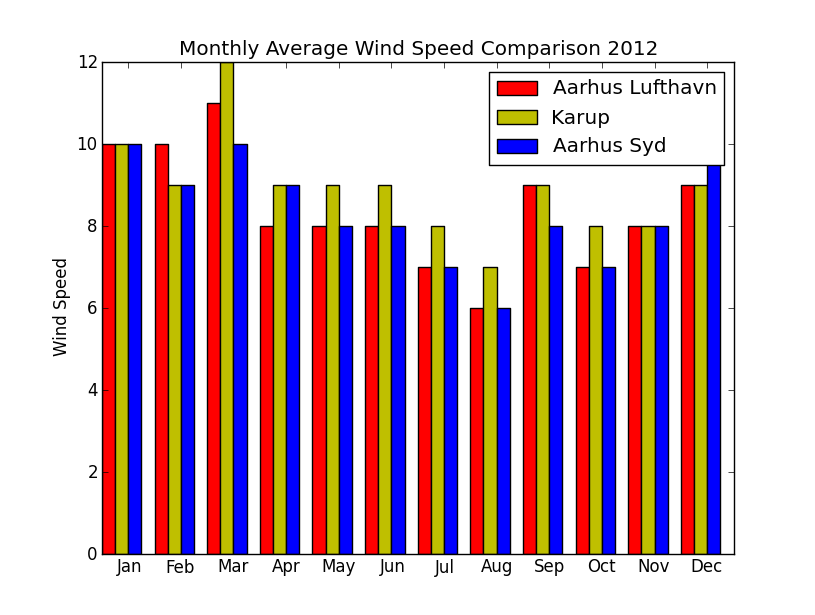
\includegraphics[width=0.85\linewidth,natwidth=898,natheight=587]{billeder/barChartMonthlyAverage.png}
\caption{Bar chart showing monthly wind speed similarity between stations in 2012}
\label{fig:barChartAverage}
\end{figure}

\begin{figure}[H]
\centering
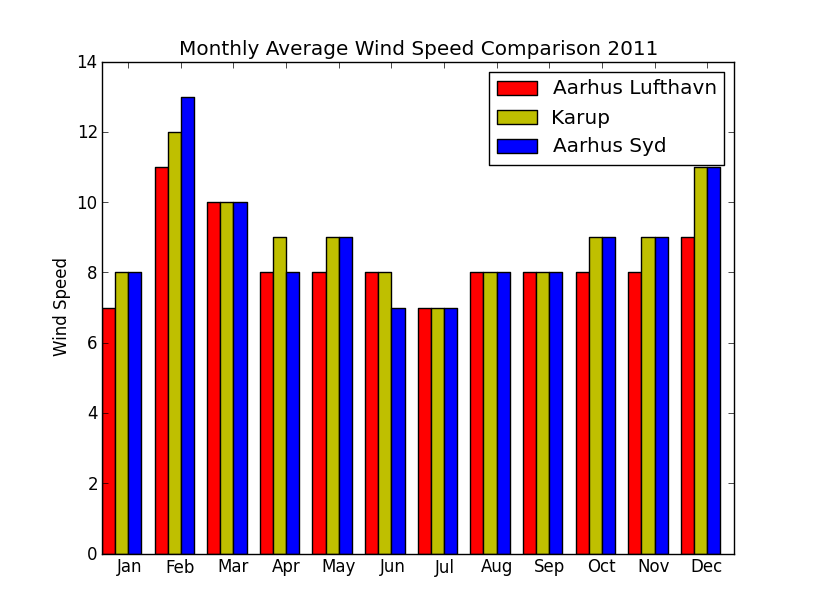
\includegraphics[width=0.85\linewidth,natwidth=898,natheight=587]{billeder/barChartMonthlyAverage2011.png}
\caption{Bar chart showing monthly wind speed similarity between stations in 2011}
\label{fig:barChartAverage2011}
\end{figure}

\begin{figure}[H]
\centering
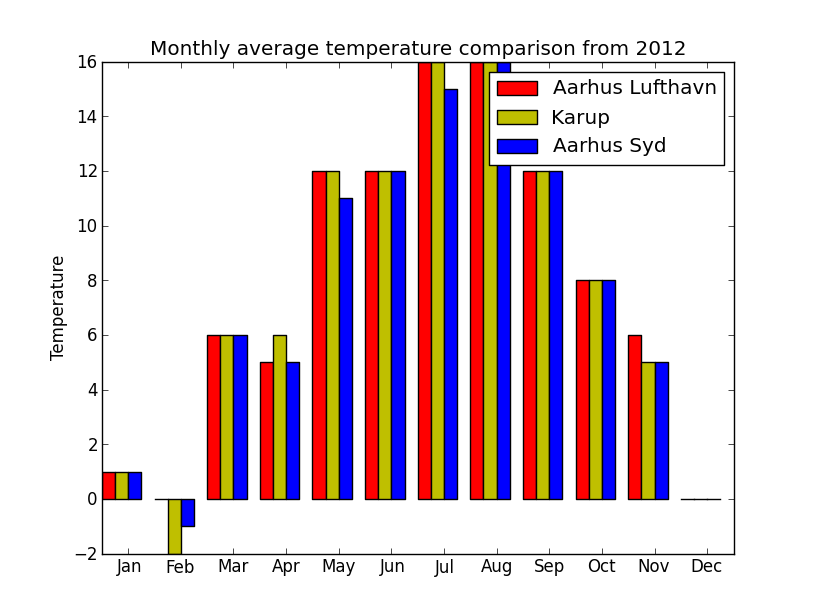
\includegraphics[width=0.85\linewidth,natwidth=898,natheight=587]{billeder/barChartMonthlyTemperatureAverage.png}
\caption{Bar chart showing monthly temperature similarity between stations in 2012}
\label{fig:barChartTempAverage}
\end{figure}

\begin{figure}[H]
\centering
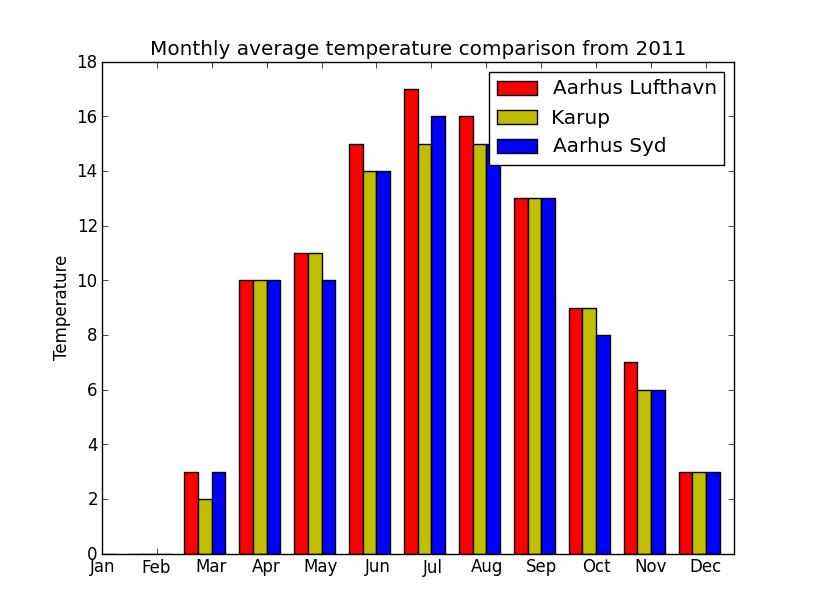
\includegraphics[width=0.85\linewidth,natwidth=898,natheight=587]{billeder/barChartMonthlyAverageTemperature2011.png}
\caption{Bar chart showing monthly temperature similarity between stations in 2011}
\label{fig:barChartMonthlyAverageTemperature2011}
\end{figure}

\begin{figure}[H]
\centering
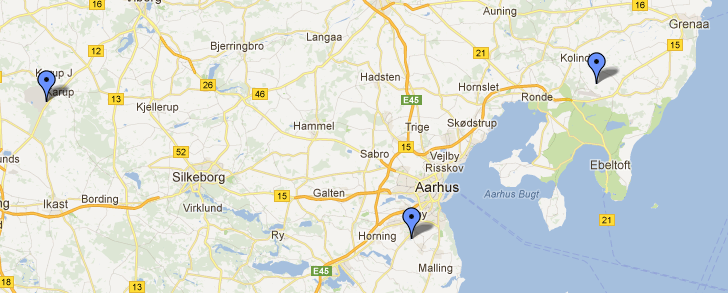
\includegraphics[width=0.85\linewidth,natwidth=898,natheight=587]{billeder/KarupAarhusSydOgLufthavn.png}
\caption{Weather stations placed close to each other}
\label{fig:closeStations}
\end{figure}

\begin{figure}[H]
\centering
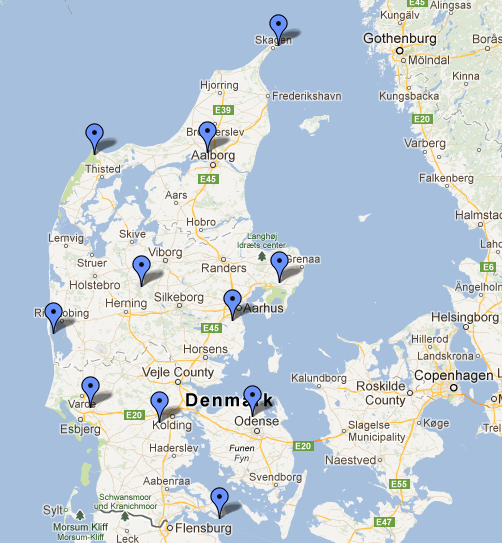
\includegraphics[width=0.85\linewidth,natwidth=898,natheight=587]{billeder/stations4average.png}
\caption{Selected weather stations in DK1}
\label{fig:stations4average}
\end{figure}

We will remove data that is obscure and is related to conditions we cannot predict. 

we need to discuss the fact that all production data stems from nordpoolspot. The impact is obscure values a times of very low consumption.